\documentclass{beamer}
\usepackage{listings}
\lstset{language=ruby,
                basicstyle=\ttfamily,
                keywordstyle=\color{red}\ttfamily,
                stringstyle=\color{orange}\ttfamily,
                identifierstyle=\color{blue},
                commentstyle=\color{gray}\ttfamily,
                morecomment=[l][\color{magenta}]{\#}
}

\usepackage[frenchb]{babel}
\usepackage[T1]{fontenc}
\usepackage[utf8]{inputenc}

\usetheme{Warsaw}
\useoutertheme{infolines}

\usepackage{amsmath}
\usepackage{amssymb}
\usepackage{amsthm}
\usepackage{stmaryrd}

\usepackage[all]{xy}

\setbeamercovered{transparent}

\begin{document}

\title{Foncteurs, Monades et Zippers}
\author{Jérémy Cochoy}
\institute{Paris RB}
\date{Février 2018}


\begin{frame}
\maketitle
\begin{center}

\includegraphics[scale=0.2]{ruby}
\end{center}
\end{frame}

\begin{frame}
  \begin{columns}[t]
  \begin{column}{5cm}
  \tableofcontents[sections={1-3}]
  \end{column}
  \begin{column}{5cm}
  \tableofcontents[sections={4-8}]
  \end{column}
  \end{columns}
\end{frame}

\begin{frame}

\begin{center}
\includegraphics[scale=0.3]{screen1.png}
\end{center}

\end{frame}

\section{Foncteurs applicatifs}

\subsection{Fonctions}
\begin{frame}[fragile]
\frametitle{Les fonctions}
\begin{block}{}
On considère des fonctions \emph{pures}:
\begin{itemize}
\item déterministe
\item sans effet de bord
\end{itemize}
\end{block}
\begin{center}

\includegraphics[scale=0.2]{fct.png}
\end{center}
\pause
\begin{block}{}
\begin{lstlisting}[language=ruby,basicstyle=\ttfamily,keywordstyle=\color{red}]
def add2(n)
  n + 2
end
\end{lstlisting}
\end{block}
\end{frame}

\subsection{Types}
\begin{frame}
\frametitle{Les types}
\begin{block}{Qu'appelons nous un type?}
Pour nous, c'est un \emph{ensemble} de valeurs.
\end{block}
\pause
\begin{exampleblock}{Exemples :}
\begin{itemize}
\item $Integer = \{-2 147 483 648, \dots, 2 147 483 647\}$
\item $NilClass = \{nil\}$
\item $Boolean = \{True, False\}$
\pause
\item $[Boolean] = \{[], [True], [False], [True, False], [False, True], \dots\}$
\end{itemize}
\end{exampleblock}
\end{frame}

\begin{frame}
\frametitle{Les types}
\begin{block}{Les fonctions sont de type : \emph{a -> b}}
\begin{itemize}
\item floor           :: Float -> Integer
\item 2.method(:+)    :: Integer -> Integer
\end{itemize}
\end{block}
\begin{block}{Les fonctions se composent}
\begin{itemize}
\item f1 :: a -> b
\item f2 :: b -> c
\item \{ |x| f2(f1(x)) \} :: a -> c
\end{itemize}
\end{block}
\end{frame}

\begin{frame}[fragile]
\frametitle{Fonctions à plusieurs paramètres}
\begin{block}{}
\begin{lstlisting}[language=ruby,basicstyle=\ttfamily,keywordstyle=\color{red}]
sum = ->(a, b) do
  a + b
end
\end{lstlisting}
\end{block}
\pause
\begin{block}{}
\begin{lstlisting}
irb> sum.(2,3)
=> 5
\end{lstlisting}
\end{block}
\pause
\begin{block}{}
\begin{lstlisting}[language=ruby,basicstyle=\ttfamily,keywordstyle=\color{red}]
irb> sum.curry.(1)
=> #<Proc:0x000000000288c3c0 (lambda)>
irb> sum.curry.(1).(2)
=> 3
\end{lstlisting}
\end{block}
\end{frame}

\begin{frame}[fragile]
\frametitle{Fonctions à plusieurs paramètres}
\begin{block}{}
\begin{lstlisting}[language=ruby,basicstyle=\ttfamily,keywordstyle=\color{red}]
sum = ->(a, b) do
  a + b
end
\end{lstlisting}
\end{block}
\begin{block}{Curryfication}
\begin{itemize}
\item sum :: (a, b) -> c
\item sum.curry :: a -> (b -> c)
\end{itemize}
\end{block}
\end{frame}

\begin{frame}[fragile]
\frametitle{Fonctions à plusieurs paramètres}
\begin{block}{}
\begin{lstlisting}[language=ruby,basicstyle=\ttfamily,keywordstyle=\color{red}]
sum = ->(a, b) do
  a + b
end
\end{lstlisting}
\end{block}
\begin{block}{Curryfication}
\begin{itemize}
\item sum :: (a, b) -> c
\item sum.curry :: a -> b -> c
\end{itemize}
\end{block}
\pause
\begin{block}{Exercice}
compose :: (a -> b) -> (b -> c) -> (a -> c)
\end{block}
\end{frame}

\subsection{Foncteurs}


\begin{frame}
\frametitle{Les foncteurs applicatifs}
\begin{block}{Un foncteur F agit sur les types ...}
\begin{itemize}
\item a => F a
\end{itemize}
\end{block}
\begin{exampleblock}{}
\begin{itemize}
\item a => [a]
\item a => Tree a
\item a => Maybe a
\end{itemize}
\end{exampleblock}

\pause

\begin{block}{... et sur les fonctions}
\begin{itemize}
\item a -> b => F a -> F b
\end{itemize}
\end{block}

\begin{exampleblock}{}
\begin{itemize}
\item fmap 2.method(:+2) :: F Int -> F Int
\item fmap floor :: F Float -> F Int
\end{itemize}
\end{exampleblock}
\end{frame}

\begin{frame}
\frametitle{Donnée dans un contexte}

\begin{center}
\includegraphics[scale=0.25]{a2fa.png}
\end{center}

\begin{block}{}
Un foncteur permet de passer d'un monde (les types a) vers un autre (les types F a).
\end{block}

\end{frame}

\begin{frame}[fragile]
\frametitle{Maybe: Une implémentation}
\begin{center}
\includegraphics[scale=0.1]{a2fa.png}
\end{center}
\begin{block}{}
\begin{lstlisting}[language=ruby,basicstyle=\ttfamily,keywordstyle=\color{red}]
class Just < Maybe
  def self.call(value)
    new [value]
  end
end
\end{lstlisting}
\end{block}
\begin{block}{}
\begin{lstlisting}[language=ruby,basicstyle=\ttfamily,keywordstyle=\color{red}]
irb> Just.(3)
=> #<Just:0x000000000359c010 @content=[3]>
\end{lstlisting}
\end{block}
\end{frame}

\begin{frame}[fragile]
\frametitle{Maybe: Une implémentation}
\begin{center}
\includegraphics[scale=0.1]{a2fa.png}
\end{center}

\begin{block}{}
\begin{lstlisting}[language=ruby,basicstyle=\ttfamily,keywordstyle=\color{red}]
class Nothing < Maybe
  def self.call()
    new []
  end
end
\end{lstlisting}
\end{block}
\begin{block}{}
\begin{lstlisting}[language=ruby,basicstyle=\ttfamily,keywordstyle=\color{red}]
irb> Nothing.()
=> #<Nothing:0x0000000002d97d38 @content=[]>
\end{lstlisting}
\end{block}
\end{frame}

\begin{frame}[fragile]
\frametitle{Maybe: Une implémentation}
\begin{block}{}
\begin{lstlisting}[language=ruby,basicstyle=\ttfamily,keywordstyle=\color{red}]
class Maybe
  private_class_method :new

  def initialize(content)
    @content = content
  end
  def from_maybe(default_value)
    return default_value if @content.empty?
    @content.first
  end
end
\end{lstlisting}
\end{block}
\end{frame}

\begin{frame}[fragile]

\begin{center}
\includegraphics[scale=0.2]{a2fa.png}
\end{center}

\begin{block}{}
\begin{lstlisting}[basicstyle=\ttfamily,keywordstyle=\color{red}]
irb> Just.(3).from_maybe
=> 3
irb> Nothing.().from_maybe
=> nil
\end{lstlisting}
\end{block}
\end{frame}


\begin{frame}
\frametitle{Functorial mapping}
On ne peut plus appliquer la fonction telle quelle :

\begin{center}
\includegraphics[scale=0.3]{wrong_type.png}
\end{center}
\end{frame}

\begin{frame}
\frametitle{Functorial mapping}
Mais le foncteur nous donne une nouvelle flèche.
\begin{center}
\includegraphics[scale=0.19]{f_fct.png}
\end{center}
\end{frame}

\begin{frame}[fragile]
  \frametitle{Implémentation de fmap}
  \begin{block}{}
    \begin{lstlisting}
def fmap(f)
  ->(box) do
    case box
    when Nothing
      return Nothing.()
    when Just
      r = f.(box.from_maybe)
      Just.(r)
    end
  end
end
    \end{lstlisting}
  \end{block}
\end{frame}

\begin{frame}[fragile]
\frametitle{Functorial mapping}
\begin{center}
\includegraphics[scale=0.1]{f_fct.png}
\end{center}
\begin{block}{}
\begin{lstlisting}[language=ruby,basicstyle=\ttfamily,keywordstyle=\color{red}]
add2 = ->(x) {x + 2}
\end{lstlisting}
\end{block}

\begin{block}{}
\begin{lstlisting}[language=ruby,basicstyle=\ttfamily]
add2.call Just.(3)
# NoMethodError (undefined method `+' for
#   #<Just:0x0000000003485280 @content=[3]>)

(fmap add2).call Just.(3)
# => #<Just:0x00000000036f8ff8 @content=[5]>
\end{lstlisting}
\end{block}
\end{frame}



\begin{frame}[fragile]
\frametitle{Dura lex sed lex}
\begin{alertblock}{Un foncteur doit respecter des lois}
\begin{itemize}
\item fmap id = id
\item fmap (p $\circ$ q) = (fmap p) $\circ$ (fmap q)

\end{itemize}
\end{alertblock}
\pause
\begin{block}{}
\begin{lstlisting}[language=ruby]
id = ->(x) {x}

(p o q) = ->(x) { p.(q.(x)) }
\end{lstlisting}
\end{block}

\pause
Un foncteur est un endofoncteur de la catégorie des types.
\end{frame}

\section{Monades}

\begin{frame}

\frametitle{Monades}
\begin{center}

\includegraphics[scale=0.5]{monad_meme.png}
\end{center}
\end{frame}

\subsection{Construction}
\begin{frame}
\frametitle{Donnée dans un contexte}

\begin{block}{}
Une monade place une valeur dans un contexte.
\end{block}

\begin{center}
\includegraphics[scale=0.3]{just3.png}
\end{center}

\begin{exampleblock}{}
L'exemple de Maybe : \verb!Just 3!
\end{exampleblock}
\end{frame}

\begin{frame}
\frametitle{Donnée dans un contexte}

\begin{block}{}
Un contexte peut aussi ne pas contenir de valeur.
\end{block}

\begin{center}
\includegraphics[scale=0.3]{nothing.png}
\end{center}
\begin{exampleblock}{}
L'exemple de Maybe : \verb!Nothing!
\end{exampleblock}
\end{frame}

\begin{frame}
\frametitle{Placer une donnée dans un contexte}

\begin{block}{L'opérateur \emph{pure}}
\begin{center}
\verb!pure :: a -> F a!
\end{center}
\end{block}

\begin{exampleblock}{Quelques cas particuliers}
	\begin{itemize}
		\item \verb!Just!
		\item \verb![] <{}<!
	\end{itemize}
\end{exampleblock}
\begin{block}{D'autres types}
	\begin{itemize}
		\item Maybe =  Nothing | Just a
		\item Tree = Leaf | Node a (Tree a) (Tree a)
		\item Either = Left a | Right b
	\end{itemize}
\end{block}
\end{frame}


\begin{frame}
\frametitle{Un traitement qui peut échouer}

\begin{center}
\includegraphics[scale=0.5]{failure.png}
\end{center}
\begin{exampleblock}{}
Une fonction de type \emph{Int -> Maybe Int}.
\end{exampleblock}
\end{frame}

\begin{frame}
\frametitle{Chainer des traitements avec échec}
\begin{block}{}
Comment composer \verb!f :: a -> M b! et \verb!g :: b -> M c! ?
\end{block}
\pause
\begin{block}{}
Si $M$ est un foncteur, on peut chainer un appel à
\verb!f :: a -> M b! avec un appel à \verb!fmap g :: M b -> M (M c)!.
\end{block}
\pause
\begin{block}{}
Que faire d'un \verb!M (M c)!?
\end{block}

\end{frame}

\begin{frame}
\frametitle{L'opérateur join}
\begin{block}{}
\begin{center}
\verb!join :: M (M a) -> M a!
\end{center}
\end{block}

\begin{center}
\includegraphics[scale=0.2]{join.png}
\end{center}
\pause
\begin{exampleblock}{}
\begin{center}
\verb!join Just.(Just.(3))!.
\end{center}
\end{exampleblock}
\end{frame}


\begin{frame}
\frametitle{L'opérateur join}
\begin{block}{}
\begin{center}
\verb!join :: M (M a) -> M a!
\end{center}
\end{block}
\medskip
\begin{center}
\includegraphics[scale=0.2]{join_nothing.png}
\end{center}
\medskip
\pause
\begin{exampleblock}{}
\begin{center}
\verb!join Just.(Nothing.())!.
\end{center}
\end{exampleblock}
\end{frame}



\begin{frame}[fragile]
\frametitle{L'opérateur \emph{join}}
\begin{center}
\includegraphics[scale=0.1]{join.png}
\end{center}
\begin{block}{Une implémentation de join :}
\begin{lstlisting}[language=ruby]
def join(bbox)
  case bbox
  when Nothing
    Nothing.()
  when Just
    bbox.from_maybe
  end
end
\end{lstlisting}
\end{block}
\end{frame}

\begin{frame}[fragile]
\frametitle{L'opérateur \emph{join}}
\begin{block}{On cherche à chainer nos traitements.}
\verb!bind :: M a -> (a -> M b) -> M b!
\end{block}

\pause

\begin{block}{Nous avons :}
\begin{itemize}
\item \verb!(fmap f) :: M a -> M (M b)!
\item \verb!join :: M (M b) -> M b!
\end{itemize}
\end{block}
\pause

\begin{block}{On peut maintenant chainer $f$ et $g$.}
\begin{lstlisting}[language=ruby]
def bind(f, v)
  join ((fmap f).(v))
end
\end{lstlisting}
\end{block}
\end{frame}

\begin{frame}
\frametitle{Récapitulatif}

\begin{block}{Une monade, c'est}

	\begin{itemize}
		\item pure :: a -> M a
		\item fmap :: (a -> b) -> (M a -> M b)
		\item join :: M (M a) -> M a
	\end{itemize}

\end{block}

\end{frame}


\subsection{Théorie}
\begin{frame}
  \begin{center}
    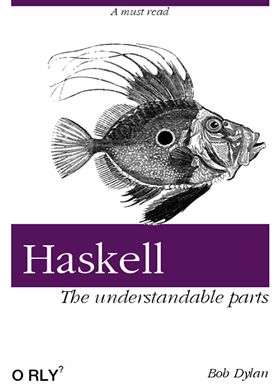
\includegraphics[scale=0.6]{haskell-the-understandable-parts}
  \end{center}
\end{frame}

\begin{frame}
\frametitle{Dura lex sed lex}
\begin{alertblock}{Une monade doit respecter des lois}
\begin{itemize}
\item \verb!pure o f $\equiv$ (fmap f) o pure!
\item \verb!join o fmap (fmap f) $\equiv$ (fmap f) o join!
\item[] \ 
\item \verb!join o fmap join   $\equiv$ join o join!
\item \verb!join o fmap pure   $\equiv$ join o pure = id!
\end{itemize}
\end{alertblock}
\end{frame}


\begin{frame}
\frametitle{Monades - Catégories}
Une monade $(T, \mu, \eta)$ est la donnée d'un
endofoncteur $T : C \rightarrow C$ et de deux
transformations naturelles $\mu : T\circ T \rightarrow T$ et $\eta : 1_C \rightarrow T$ telles que :

\[
\begin{array}{cc}
\xymatrix{
T(T(T(X))) \ar[r]^{T(\mu_X)} \ar[d]_{\mu_{T(X)}} & T(T(X)) \ar[d]^{\mu_X} \\
T(T(X)) \ar[r]_{\mu_X} & T(X) \\
}
&
\xymatrix{
T(X) \ar[r]^{\eta_{T(X)}} \ar[d]_{T(\eta_X)}  \ar@{=}[dr] & T(T(X)) \ar[d]^{\mu_X} \\
T(T(X)) \ar[r]_{\mu_X} & T(X) \\
}
\end{array}
\]
c'est à dire
$\mu \circ T\mu = \mu \circ \mu_T$
et
$\mu \circ T \eta = \mu \circ \eta_T = id_T$.

\pause
\medskip\medskip
Dans notre cas $C$ la catégorie des types.
\end{frame}

\begin{frame}
\frametitle{A chaque loi son diagramme}
\begin{alertblock}{\verb!pure! est une T.N.}
\verb!pure . f $\equiv$ (fmap f) . pure!
\end{alertblock}

\begin{block}{}
\[
\xymatrix{
X \ar[r]^{f} \ar[d]_{\eta_X} & Y \ar[d]^{\eta_Y} \\
T(X) \ar[r]_{T(f)} & T(Y) \\
}
\]
\end{block}

\end{frame}

\begin{frame}
\frametitle{A chaque loi son diagramme}
\begin{alertblock}{\verb!join! est une T.N.}
\verb!join o fmap (fmap f) $\equiv$ (fmap f) o join!
\end{alertblock}

\begin{block}{}
\[
\xymatrix{
T(T(X)) \ar[r]^{T(T(f))} \ar[d]_{\mu_{X}} & T(T(Y)) \ar[d]^{\mu_{Y}} \\
T(X) \ar[r]_{T(f)} & T(Y) \\
}
\]
\end{block}

\end{frame}


\begin{frame}
\frametitle{A chaque loi son diagramme}
\begin{alertblock}{Associativité}
\verb!join o fmap join $\equiv$ join o join!
\end{alertblock}

\begin{block}{}

\[
\xymatrix{
T(T(T(X))) \ar[r]^{T(\mu_X)} \ar[d]_{\mu_{T(X)}} & T(T(X)) \ar[d]^{\mu_X} \\
T(T(X)) \ar[r]_{\mu_X} & T(X) \\
}
\]
\end{block}

\begin{block}{}
\begin{center}
$\mu \circ T\mu = \mu \circ \mu_T$
\end{center}
\end{block}

\end{frame}

\begin{frame}
\frametitle{A chaque loi son diagramme}
\begin{alertblock}{Existence d'un neutre}
\verb!join o fmap pure $\equiv$ join o pure = id!
\end{alertblock}

\begin{block}{}
\[
\xymatrix{
T(X) \ar[r]^{\eta_{T(X)}} \ar[d]_{T(\eta_X)}  \ar@{=}[dr] & T(T(X)) \ar[d]^{\mu_X} \\
T(T(X)) \ar[r]_{\mu_X} & T(X) \\
}
\]
\end{block}

\begin{block}{}
\begin{center}
$\mu \circ T \eta = \mu \circ \eta_T = id_T$
\end{center}
\end{block}

\end{frame}

\section{Applications In Real Life}
\begin{frame}
  \frametitle{Et dans la vraie vie ?}
  \begin{alertblock}{}
  \begin{center}
    Tout ça, à quoi ça sert?
  \end{center}
  \end{alertblock}
\end{frame}

\subsection{Monade de listes}
\begin{frame}
  \frametitle{Calculs non déterministes}
  \begin{center}
    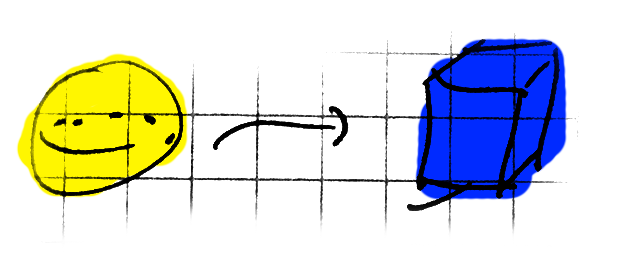
\includegraphics[scale=0.2]{deter-geometric}
  \end{center}
  \begin{block}{}
    \begin{itemize}
      \item Déterministe: Calcul produisant une valeur.
    \end{itemize}
  \end{block}
  \medskip
  \begin{center}
    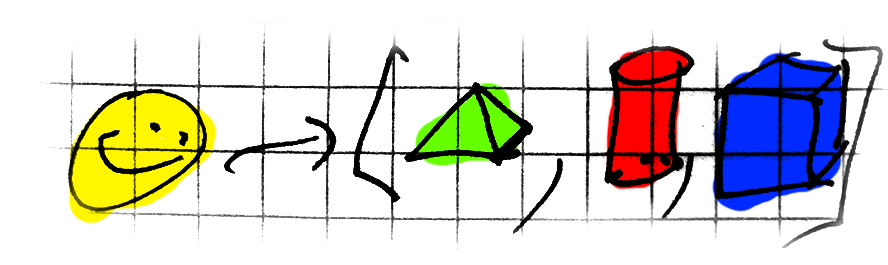
\includegraphics[scale=0.2]{non-deter-geometric}
  \end{center}
  \begin{block}{}
    \begin{itemize}
      \item Non déterministe: Calcul produisant plusieurs valeurs.
    \end{itemize}
  \end{block}
\end{frame}

\begin{frame}[fragile]
  \frametitle{Quelques exemples}
  \begin{center}
    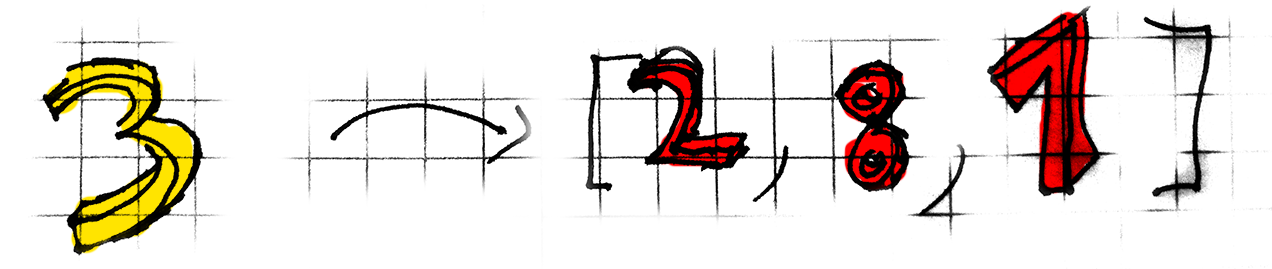
\includegraphics[scale=0.2]{multiple-res.png}
  \end{center}
  \begin{block}{}
    \begin{lstlisting}[language=ruby]
powers = ->(n) do
  [n, n*n, n*n*n]
end
    \end{lstlisting}
  \end{block}
  \begin{block}{}
    \begin{lstlisting}[language=ruby]
neighbors = ->(n) do
  [n-1, n+1]
end
    \end{lstlisting}
  \end{block}
\end{frame}

\begin{frame}[fragile]
  \frametitle{Implémentation de fmap}
  \begin{exampleblock}{C'est tout simplement \verb!Array\#map!}
    \begin{center}
      $[1, 2, 3] {\xrightarrow{\text{.map(f)}}} [f(1), f(2), f(3)]$
    \end{center}
  \end{exampleblock}
  \medskip
  \begin{block}{}
    \begin{lstlisting}[language=ruby]
def fmap(f)
  ->(list) { list.map(f) }
end
    \end{lstlisting}  
  \end{block}
\end{frame}

\begin{frame}[fragile]
  \frametitle{Join}
  \begin{center}
    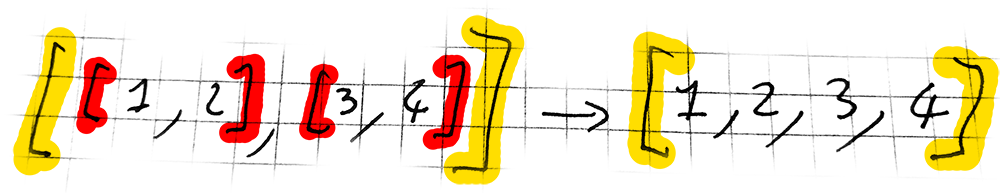
\includegraphics[scale=0.2]{flatten}
  \end{center}
  \begin{block}{\verb!join!}\begin{lstlisting}[language=ruby]
def join(llist)
  llist.flatten(1)
end
    \end{lstlisting}  
  \end{block}
\end{frame}

\begin{frame}[fragile]
  \frametitle{Monkey patch pour bind}
  \begin{center}
    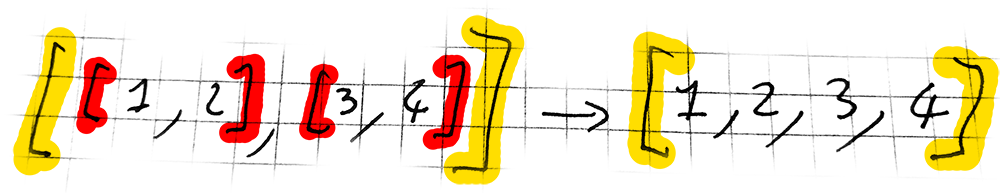
\includegraphics[scale=0.2]{flatten}
  \end{center}
  \begin{block}{\verb!bind!}\begin{lstlisting}[language=ruby]
class Array
  def bind(&f)
    return self.map(&f).flatten(1)
  end
end
    \end{lstlisting}  
  \end{block}
\end{frame}

\begin{frame}[fragile]
  \frametitle{Monade de listes}
  \begin{exampleblock}{Example d'utilisation}
    \begin{lstlisting}[language=ruby]
irb> [42].bind(&neighbors).bind(&neighbors)
=> [40, 42, 42, 44]
irb> [2].bind(&powers).bind(&powers)
=> [2, 4, 8, 4, 16, 64, 8, 64, 512]
irb> [42].bind(&neighbors).bind(&powers)
=> [41, 1681, 68921, 43, 1849, 79507]
irb>[42].bind { |x| [x, -x] }.bind(&neighbors)
=> [41, 43, -43, -41]
    \end{lstlisting}
  \end{exampleblock}
\end{frame}

\subsection{La Monade Maybe de Ruby}

{
\setbeamercolor{background canvas}{bg=black}
\begin{frame}
  \frametitle{La monade \verb!nil!}
  \begin{center}
    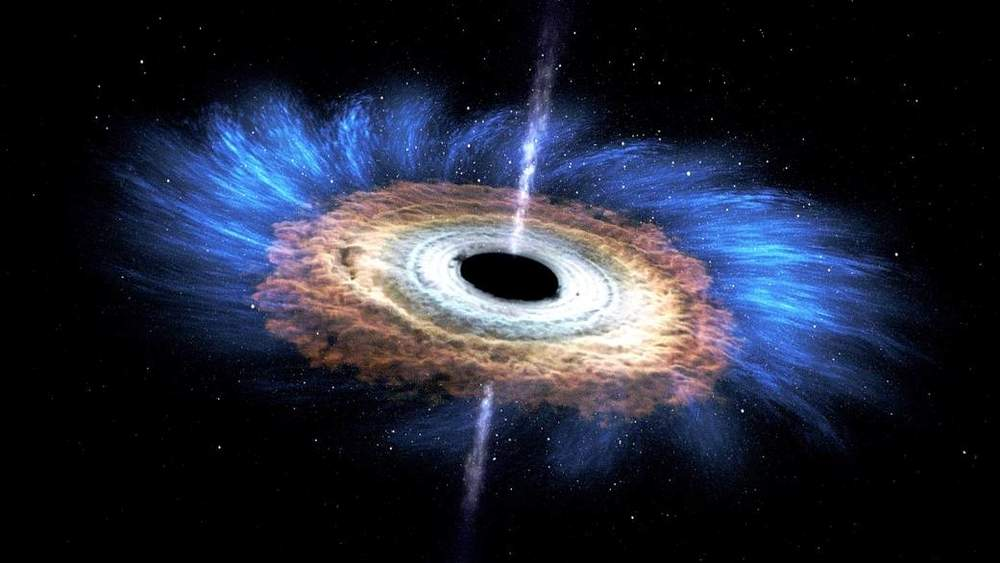
\includegraphics[scale=0.8]{blackhole}
  \end{center}
  \begin{alertblock}{En ruby Maybe s'appelle \verb!nil!}
  Union disjointe $a \bigsqcup \{nil\}$.
  \end{alertblock}
\end{frame}
}
{
\setbeamercolor{background canvas}{bg=black}
\begin{frame}[fragile]
  \frametitle{La monade \verb!nil!}
  \begin{center}
    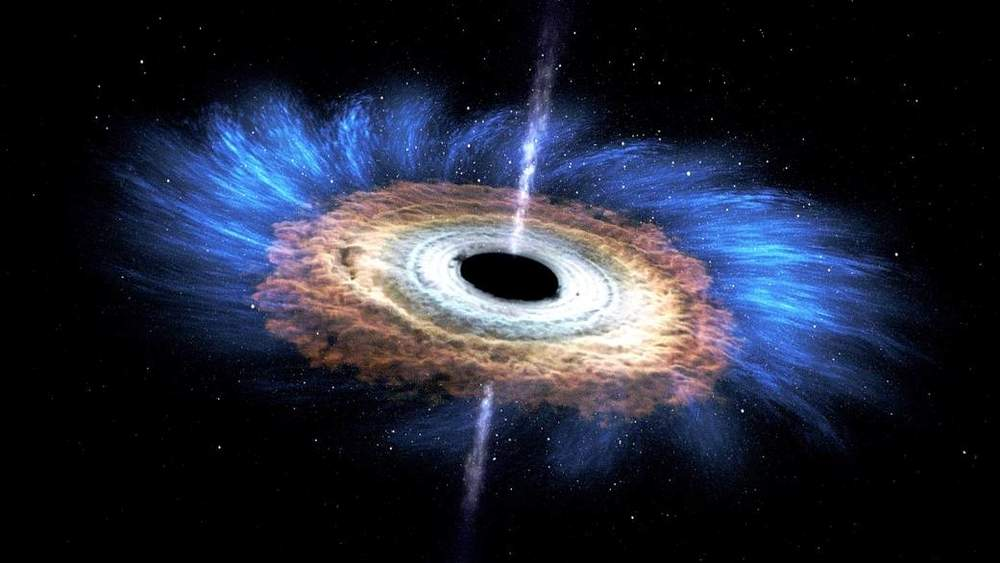
\includegraphics[scale=0.4]{blackhole}
  \end{center}
  \begin{block}{Opérateur bind \verb!\&.!}
    \begin{lstlisting}[language=ruby]
some_computation(42)&.get_value("bidirectional")
    \end{lstlisting}
  \end{block}
  \begin{block}{Opérateur bind \verb!\&.!}
  \begin{itemize}
  \item  \&. :: $a \bigsqcup \{nil\}$ -> (a -> $b \bigsqcup \{nil\})$ -> $b \bigsqcup \{nil\}$
  \item bind :: M a -> (a -> M b) -> M b
  \end{itemize}
  
  \end{block}
\end{frame}
}

\begin{frame}[fragile]
  \frametitle{On aurait aussi pu parler de...}
\begin{columns}[T]
  \begin{column}{0.5\textwidth}
    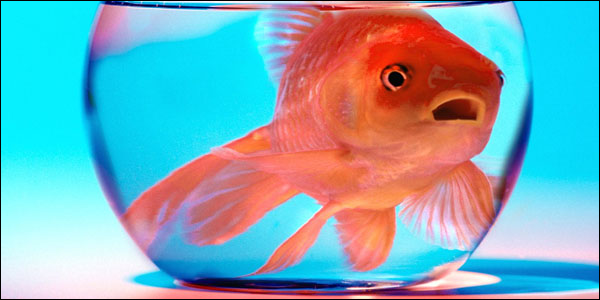
\includegraphics[scale=0.3]{goldfish}
  \end{column}
  \begin{column}{0.5\textwidth}
    \begin{itemize}
      \item Left/Right Fish et Bind
      \item List comprehension
      \item Monades transformeurs
      \item Comonades et zippers
      \item Application aux automates cellulaires
    \end{itemize}
  \end{column}
\end{columns}
\end{frame}

\begin{frame}
  \frametitle{Qui suis-je?}
  \begin{columns}[T]
    \begin{column}{0.5\textwidth}
      \begin{center}
        \includegraphics[scale=0.06]{techgate}
      \end{center}
      \begin{center}
         
\includegraphics[scale=0.25]{social-networks}
      \end{center}
    \end{column}
    \begin{column}{0.5\textwidth}
      \begin{block}{Dr. Jérémy Cochoy}
      \begin{center}
      	 jeremy.cochoy@gmail.com
         \verb!http://techgate.fr!
      \end{center}
      \end{block}
      \begin{block}{Backend Developper}
        \begin{center}
          
\includegraphics[scale=0.4]{klaxit}
        \end{center}
      \end{block}
    \end{column}
  \end{columns}
\end{frame}

\begin{frame}
  \begin{center}
    \includegraphics[scale=1]{chaton.png}
  \end{center}
  \begin{center}
    Merci pour votre attention!
  \end{center}
\end{frame}

\end{document}
